\documentclass[a4paper]{article}

  \usepackage{fullpage} % Package to use full page
  \usepackage{parskip} % Package to tweak paragraph skipping
  \usepackage{tikz} % Package for drawing
  \usepackage{amsmath}
  \usepackage{siunitx} % Package for scientific units
  \usepackage{amsfonts}
  \usepackage{amssymb}
  \usepackage{hyperref}
  \usepackage[utf8]{inputenc}
  \usepackage[english]{babel}
  \usepackage{multicol}
  \usepackage{graphicx} % Package for including images
  \graphicspath{ {./images/} }
  
  \newcommand\tab[1][0.5cm]{\hspace*{#1}}
  
  \title{Lab 2}
  \author{Adrian Darian}
  \date{9/14/2020}
  
  \begin{document}
  
\maketitle
  
\section*{Discussion Section 2}

\section*{Instructions:}
This week you will use R to study the classical probability problem of sampling without replacement from an urn. \\

You will receive some basic guidance in R from your TAs and a piece of code that you will only need to slightly modify.  You are welcome to work alone or in small groups but everyone is responsible for turning in their own code/assignment. \\

This week, you are responsible for submitting: \\

\begin{itemize}
    \item Your modified R script.
    \item A written report as a PDF which shows the plots you have created in R and answers the questions below. \\
    Note:  If you can not submit as a PDF you should get permission for a different fileformat from your TA. \\
\end{itemize}

Simply providing the correct answer, without justification, is not considered complete. For credit you \textbf{must} either show you steps (if it’s a calculation problem) or explain/justify your reasoning (if it’s a short answer problem).

\section*{Assignment:}
This Lab considers the following scenario: \\

You have an urn with a total of 7 balls: 3 black balls and 4 red balls. You will draw 3 ballsfrom this urn \textbf{without replacement}. Estimate the probability of drawing 0,1, 2 or 3 blackballs and compare this estimate to the true probabilities.

\begin{itemize}
    \item[1.] Calculate the true probabilities in this scenario.  (This will be in your written report.The code you received provides a lot of reasoning in the comments.)
    \item[2.] Either modify the code you were given (or if you like create your own) to simulate this scenario. (This code will be submitted as an R script.)
    \item[3.] Provide output from your code (the figures comparing both probabilities) forat least these two different scenarios: \\
    \begin{itemize}
        \item[(a)] numTrials=$10^2$ \\
        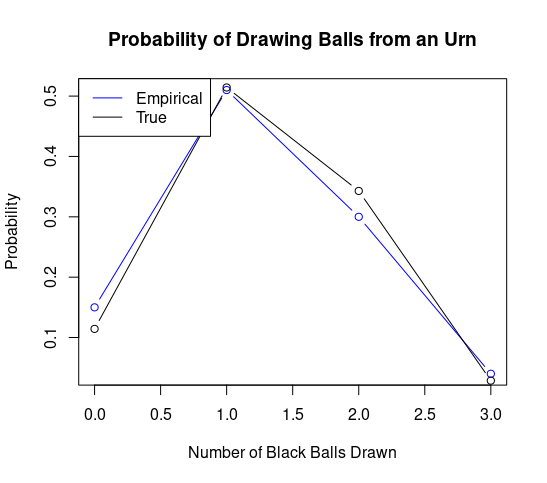
\includegraphics{Rplot-100.png} \\ 
        \item[(b)] numTrials=$10^4$ \\
        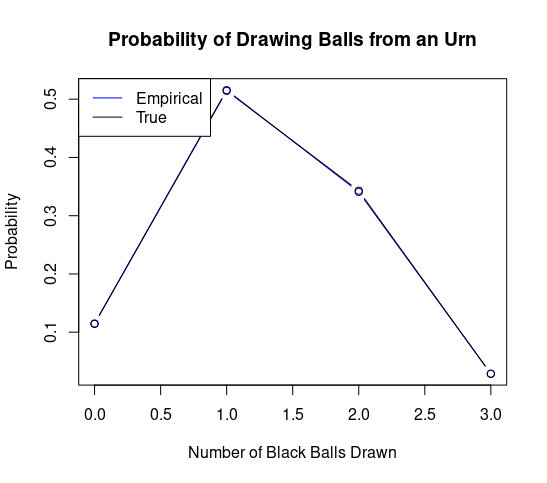
\includegraphics{Rplot-10000.png} \\ 
    \end{itemize}
    \item[4.] A short explanation of what is shown in your graphs and what you have learned from this exercise. (Example:  Do you feel you agree well with the theoretical results?  Which one is better?  How many trials do you think you need to get a “good” agreement to the true probability?) \\
    \hbox to 2cm{} \\ 
    \tab The graphs shown above are taken at 2 differen trial intervals the first being $10^2$ and the second being $10^4$. While both look similar one can easily tell which graph had more trial runs before drawing the results. As an experiment conducts its computation more and more the end results continue to become more finite to the point where there is nothing but an exact answer for the given scenario. 
    \item[5.] Extra Credit (1 Point): (There is no single right answer to this next question!) If you did not know the true probabilities for this experiment how would you decide your simulations had considered enough trials. \\
    \hbox to 2cm{} \\
    \tab On average if you run a test 100 time. Your bound to get some kinda of results and if you see it changing crazily during those 100 then it hasn’t found it’s break even point. So run it 1,000 times. And try again and see 
\end{itemize}
  
\end{document}